The aim of the experiment was to gather forearm surface EMG data in
real-time, and to relate it to $(a)$ the type of grasp applied by the
subject, $(b)$ the force applied by the subject while grasping.

\subsubsection{General setup description}

The experiment consisted of freely, repeatedly pressing a SpaceControl
OFTS force/torque sensor \cite{...} along the large face. Four
different ways of pressing were allowed: opposing the thumb and index,
the thumb and middle, the thumb and ring or the thumb and all other
fingers, at different speeds and with varying force. Four force-sensor
resistors were applied on the subject's hand fingertips (thumb, index,
middle and ring), in order to be able to detect which grasp type was
used at each instant of time. At the same time, $10$ forearm surface
EMG electrodes were applied to the subject's forearm, in order to
gather information about the muscle activation. Figure \ref{fig:setup}
shows some parts of the setup.

\begin{figure*}[!ht] \centering
  \begin{tabular}{ccc}
    \includegraphics[height=0.16\textheight]{figs/OFTS} &
    \includegraphics[height=0.16\textheight]{figs/ottobock} &
    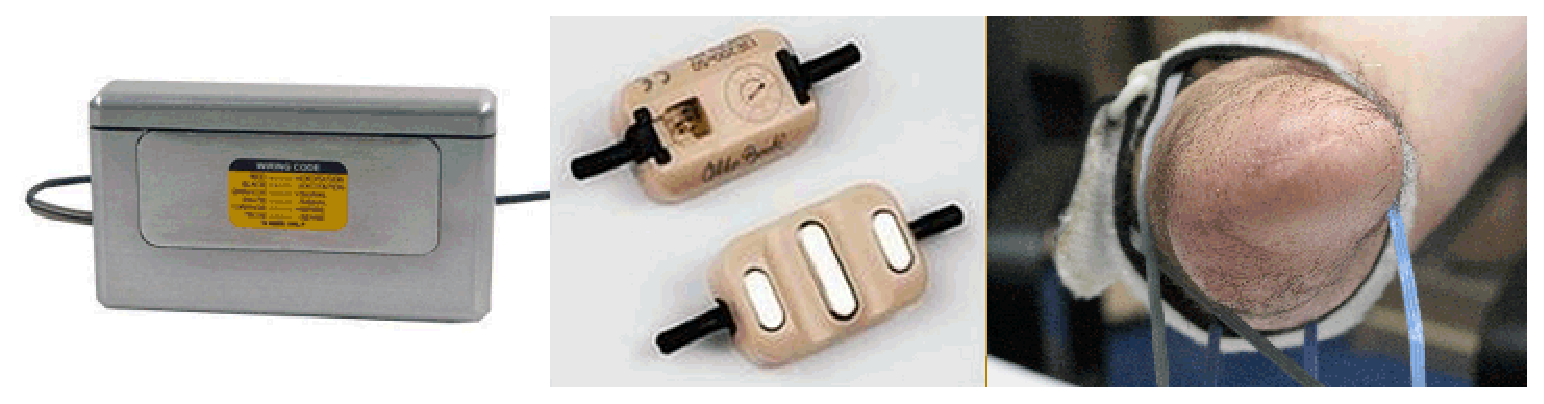
\includegraphics[height=0.16\textheight]{figs/setup} \\
    $(a)$ & $(b)$ & $(c)$ \\
  \end{tabular}
  \caption{The experimental setup. $(a)$ The SpaceControl OFTS
    force/torque sensor, large face up. $(b)$ An Otto Bock 13E200=50
    surface EMG electrode, with the amplification gauge (upper part of
    the Figure) and the three metallic contacts (lower part). $(c)$
    The arm of the subject with the EMG electrodes fitted and held in
    place by elastic bands. Electrodes cables are wired in a box and
    then directed to a National Instruments PCI-6023E analogic/digital
    conversion card (not shown).}
  \label{fig:setup}
\end{figure*}

Numerical data from the EMG and fingertip sensors were gathered at a
sampling rate of $256$Hz using a National Instruments DAQ PCI-6023E
analogic/digital conversion card \cite{...}, mounted on a fast PC
equipped with Windows XP. Data coming from the OFTS sensors was
gathered via the serial port. We ensured that the sampling rate was
high enough and that the card and serial port would respond properly
when requested for data. The data were subsequently synchronised and
saved onto files.

\subsubsection{EMG signal and electrode placement}

The $10$ EMG electrodes were applied to the subject's right forearm,
held in place by elastic bands. The electrodes were
double-differential Otto Bock 13E200=50 models \cite{...}, each one
gifted with an amplification gauge ranging from $2000$ to $100000$
times. Initial qualitative experiments revealed that a safe setting
for the amplification gauge was in the middle of the range,
corresponding to about $14000$ times. This is in agreement with the
EMG signal amplitude predicted in the related literature (see, e.g.,
\cite{deluca}), that is about $100 \mu V$ on average: the voltages our
DAQ card read ranged from slightly more than $0V$ to $3V$.

Six of the electrodes were placed in pairs along the lower face
of the forearm, whereas four of them were applied in pairs on the
upper face. The initial positioning of the electrodes was chosen
following an anatomical guideline \cite{...} in order for them to lie
approximately on top of the muscles which elicit finger movements. As
well, we were inspired by the placement description in \cite{smagt},
which proved to be optimal for Support Vector Machine classification
of hand postures.

As far as the EMG signal is concerned, it must be remarked that it is
subject to remarkable changes depending on, at least, four orders of
factors:

\begin{enumerate}

  \item \emph{the subject.} All forearms are different from one
    another in shape, size and power.

  \item \emph{arm posture.} Besides finger movements and grasping, the
    forearm muscles are also involved in the motion of the arm. The
    EMG signal is therefore likely to change if the forearm is moved
    during signal acquisition, for example when switching from
    pronation to supination.

  \item \emph{electrode placement.} The intensity and quality of the
    EMG signal depends upon a correct placement of the electrode over
    a muscle. In principle, each electrode should be placed over a
    single muscle, precisely on top of the muscle belly, halfway the
    length of the muscle, and always exactly in the same place.

  \item \emph{muscle fatigue.} As the muscles are used more and more,
    continually, fatigue changes the RMS of the EMG signal, calling
    for continual adaptation, at least over a reasonable set of
    different fatigue conditions.

\end{enumerate}

As far as the first problem is concerned, since in a real setting one
person only is expected to train and wear the prosthesis, we have not
investigated multi-subject feasibility of the approach, concentrating
on one subject only, male, aged $35$ and fully able-bodied. Of course,
further investigation is required to check whether the approach can be
transferred to real amputees, by exploiting the residual potential
muscular activation left in their forearm stump. Moreover, independent
multi-subject analysis will have to be carried on, in order to check
that the described approach works with the same accuracy results for
any human being.

In order to overcome the second problem, we instructed the subject to
keep the arm still and relaxed on a table in a confortable position,
with the palm orthogonal to the plane of the table.

Lastly, as far as muscle fatigue and electrode displacement are
concerned: in general, electrodes \emph{cannot} be expected to exactly
lie in the very same position every time the prosthesis is used;
moreover, in a preliminary round of experiments, muscle fatigue was
clearly perceived by the subject during the experiment. In this
framework, the only possibility to overcome these problems is to
explicitly take them into account, gathering enough data to be able to
train the machine under different conditions of electrode displacement
and muscular fatigue.

We then organised the experiment as follows: the subject was
instructed to continually grasp the sensor over a period of time of
three to four minutes; then he was allowed to rest for about two
minutes. This was called a \emph{session}. It was expected that muscle
fatigue would appear already during one session.

Three sessions were gathered without taking the elastic bands off the
subject's forearm, in order \emph{not} to have electrode displacement
within a set of three sessions, that we called a \emph{group}. After
each group, the electrodes and bands were removed and the subject was
allowed for a much longer period of rest, ranging from half an hour to
one hour. During resting in-between groups, the subject could get back
to his normal muscular activity.

Five groups were then gathered during one day; and this procedure was
entirely repeated during another day. This procedure would allow us to
examine a relevant amount of data, gathered along a relatively long
period of time and inder different conditions of muscle fatigue
(within one session) and electrode displacement (between groups).

As an example, Figure \ref{fig:drift} shows the output of electrode
$8$ during three different sessions: $1$ and $2$, belonging to the
same group, and $7$ (moving average over about $10$ seconds). One can
notice strong low-frequency components, essentially drifts due to
muscle fatigue.

\begin{figure*}[!ht] \centering
  \begin{tabular}{ccc}
    \includegraphics[width=0.32\textwidth]{figs/el8_movingAvg_s1} &
    \includegraphics[width=0.32\textwidth]{figs/el8_movingAvg_s2} &
    \includegraphics[width=0.32\textwidth]{figs/el8_movingAvg_s7} \\
    session $1$ & session $2$ & session $7$ \\
  \end{tabular}
  \caption{Typical behaviour of an electrode signal over different
  sessions (moving average over about $10$ seconds. Drifting can be
  clearly seen in the signal, due to muscle fatigue.}
  \label{fig:drift}
\end{figure*}

\subsubsection{Force applied during the grasp}

The OFTS force/torque sensor would output a (negative) numerical value
ranging from $0$ to about $5000$, expressed in fiftieths of a
Newton. After normalisation, the range would be between $0N$ and
$50N$.

\subsubsection{Type of grasp}

The values output by the $4$ force resistor sensors applied onto the
subject's fingertips were monitored in order to understand which kind
of grasp the subject was applying to the sensor. A threshold was
experimentally decided, above which the finger would be in contact
with the sensor. Using this technique, for each instant in time one of
five possible categories was established: $0$, no action; $1$,
grasp by opposing the thumb and index finger; $2$, opposing thumb and
middle; $3$ thumb and ring; and lastly, $4$ grasp by opposing the
thumb and all other fingers.

It must be remarked here that the EMG signal would be altered
immediately at the onset of finger movement, which our setup was
unable to detect. This would result in potential noise in the
categorisation of category $0$.

Figure \ref{fig:targets} shows typical values of the OFTS sensor and
the related categories. One can clearly see that the applied force is
in general higher when grasp type $4$, all fingers involved, is used,
as expected.

\begin{figure*}[!ht] \centering
  \begin{tabular}{cc}
    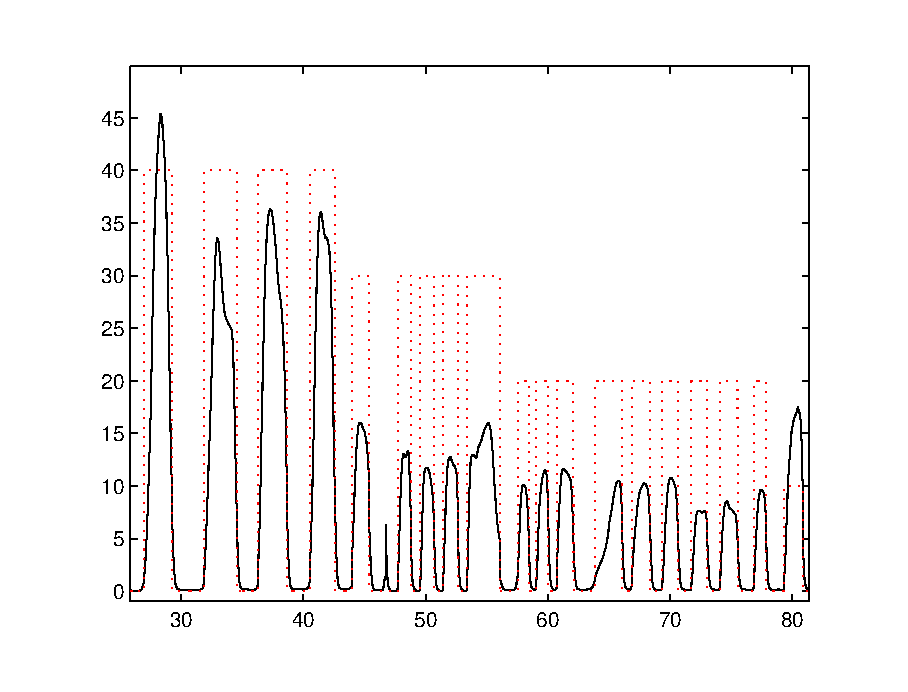
\includegraphics[width=0.45\textwidth]{figs/targets_zoom1} &
    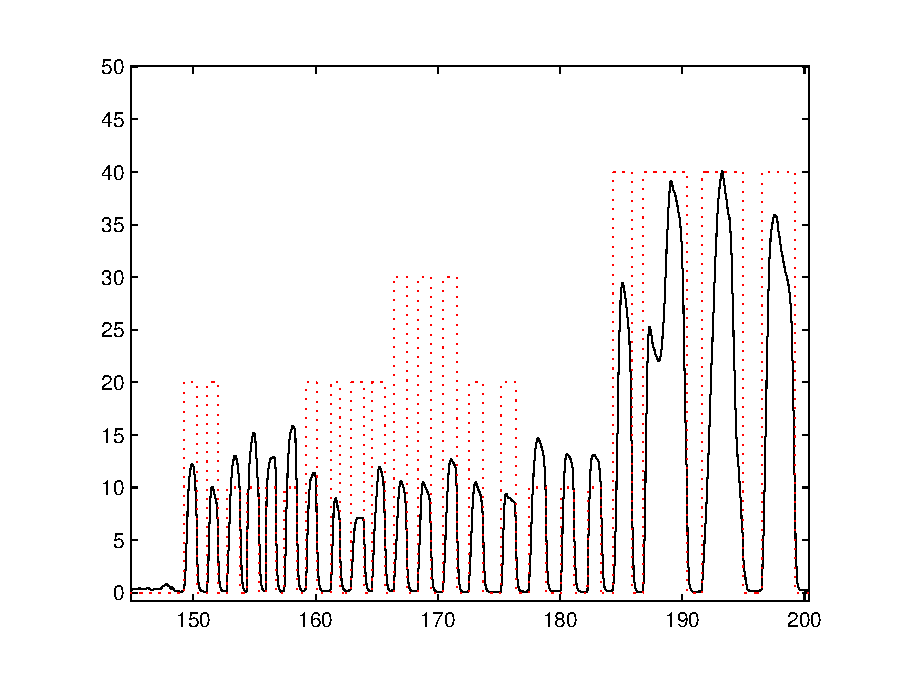
\includegraphics[width=0.45\textwidth]{figs/targets_zoom2} \\
  \end{tabular}
  \caption{Typical values output by the OFTS sensor (black line), and the
    categories evaluated from the fingertip sensors values (red
    line). The Figures are zooms of the same session.}
  \label{fig:targets}
\end{figure*}
